\documentclass[a4paper,10pt]{article}

\usepackage[english]{babel}
\usepackage{graphicx}
\usepackage{placeins}
\usepackage[colorlinks, linkcolor=black, citecolor=black, urlcolor=black]{hyperref}
\usepackage{geometry}
\geometry{tmargin=3cm, bmargin=2.2cm, lmargin=2.2cm, rmargin=2cm}
\usepackage{todonotes} %Used for the figure placeholders

% Your name and student number must be filled in on the title page found in
% titlepage.tex.

\begin{document}
\begin{titlepage}
    \newpage
    \thispagestyle{empty}
    \frenchspacing
    \hspace{-0.2cm}
    
\includegraphics[height=3.4cm]{sedes}
    \hspace{0.2cm}
    \rule{0.5pt}{3.4cm}
    \hspace{0.2cm}
    \begin{minipage}[b]{8cm}
        \Large{Katholieke\newline Universiteit\newline Leuven}\smallskip\newline
        \large{}\smallskip\newline
        \textbf{Department of\newline Computer Science}\smallskip
    \end{minipage}
    \hspace{\stretch{1}}
    \vspace*{3.2cm}\vfill
    \begin{center}
        \begin{minipage}[t]{\textwidth}
            \begin{center}
                \LARGE{\rm{\textbf{\uppercase{Document Processing}}\\ADD
                application}}\\
                \Large{\rm{Software Architecture (H09B5a and H07Z9a) -- 
                Part 2a}}
            \end{center}
        \end{minipage}
    \end{center}
    \vfill
    \hfill\makebox[8.5cm][l]{%
        \vbox to 7cm{\vfill\noindent
            {\rm \textbf{Student A (r123456)}}\\
            {\rm \textbf{Student B (r987654)}}\\[2mm]
            {\rm Academic year 2014--2015}
        }
    }
\end{titlepage}


\tableofcontents
\newpage

\section{Domain analysis}\label{sec:domain}
\subsection{Domain model}
This section shows the domain model.

\begin{figure}[h]
    \centering
    %\includegraphics[width=0.8\textwidth]{}
	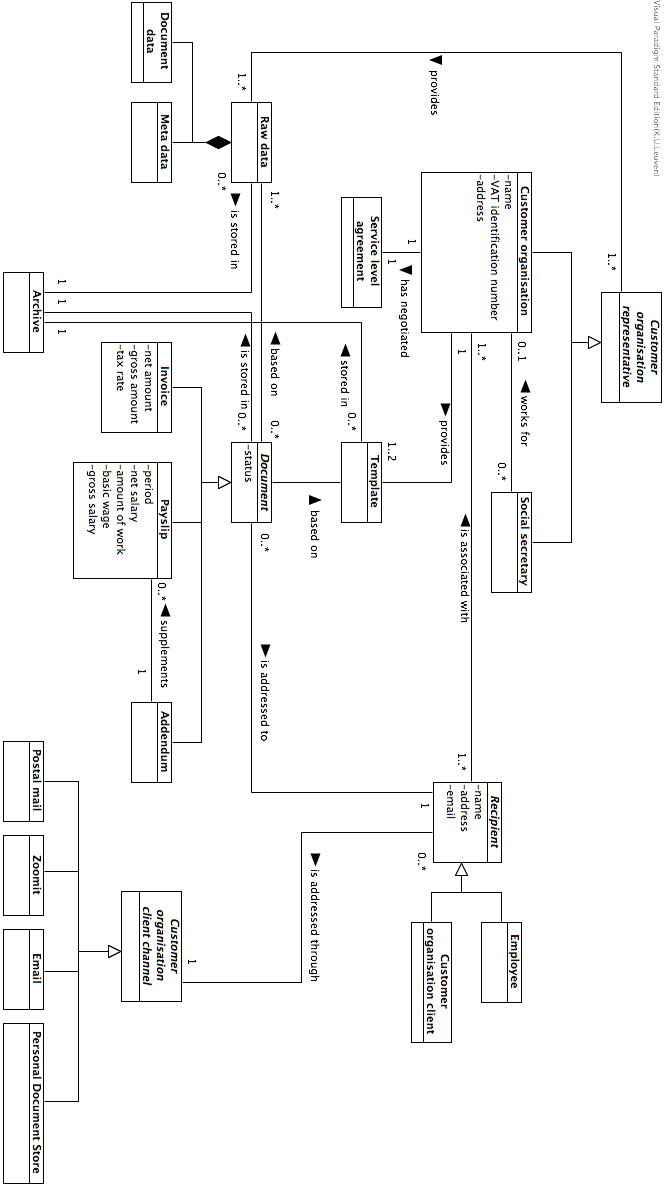
\includegraphics[width=0.6\textwidth]{eDocs_domain_model.png}
    \caption{The domain model for the system.}\label{fig:domain_model}
\end{figure}
\FloatBarrier
\subsection{Domain constraints}
In this section we provide additional domain constraints.

\begin{itemize}
    \item A Recipient should have at most one personal document store.
    \item A Recipient should get a specific document over one channel.
    \item The System must first generate a document before it can archive it.
    \item If a document is stored in the archive, the raw data on which it is based should also be stored in the archived. 
    \item An Employee can receive only payslips.
    \item A Customer organization client can receive only invoices.
    \item \emph{Employee} and \emph{Customer organization client} are roles. They might be taken on by the same person.
    \item There are two possible ways data from a Customer organization can be provided. The first way is the Customer organization providing the data for both invoices and payslips. The alternative consists of the Customer organization providing only the data for invoices while the data for payslips is being provided by one or more Social secretaries.
    \item Each Customer organization must fill in a separate template for payslips and invoices.
    \item A Personal document store can only show documents that are in the archive.
    \item It should be possible for a Recipient's Personal document store to show all of the Recipient's documents that have previously been archived.
    \item The archive contains all of the documents that have been generated.
\end{itemize}

\subsection{Glossary}
In this section, we provide a glossary of the most important terminology used
in this analysis.

\begin{itemize}
	\item \textbf{Customer organisation}: an organisation that outsources its document processing for payslips and/or
invoices to eDocs.
	\item \textbf{Invoice}: a commercial document issued for the sale of goods and/or services from a seller to a buyer.
	\item \textbf{Payslip}: a document sent out by companies to their employees that describes how their salary for a certain
period is calculated.
\item \textbf{Raw data}: the unformatted information that is represented in a document.
\item \textbf{Recipient}: a person or organisation that receives a document, e.g. an employee of a customer organisation
or a client subscribed to the services of a customer organisation.
	\item \textbf{Employee}: a Receiver of payslips send by a Customer organization representative.
    \item \textbf{Customer organization client}: a Receiver of invoices send by a Customer organization.
    \item \textbf{Archive}: a logical place where the received raw data and generated documents are stored.
    \item \textbf{Meta data}: part of the raw data that specifies the addressing method and address for a specific Recipient.
    \item \textbf{eDocs administrator}: an employee of eDocs that supervises the system infrastructure.
    \item \textbf{Customer organization representative}: a(n) (employee of a) company  who can deliver raw data in the name of the Customer organization.
    \item \textbf{Social secretary}: representative of the Customer organization it works for.
    \item \textbf{Service Level Agreement}: a contract between the company eDocs and a customer organization or between the eDocs company and an organization to which eDocs outsources services, specifying the services that have to be provided by both parties and the conditions under which it is valid. 
    \item \textbf{template}: a predefined textual structure on which the generated documents are based.
    \item \textbf{Personal document store}: a channel provided by the eDocs company through which a receiver can consult all documents for which he or she is the receiver.
    \item \textbf{Channel}: a medium over which Recipients can receive documents.
    \item \textbf{Addendum}: a document complementing a previously sent payslip.
    \item \textbf{Document data}: the part of the raw data that specifies the contents of a document.
\end{itemize}

\section{Functional requirements}\label{sec:functional}
\subsection*{Use case model}

\begin{figure}[!htp]
    \centering
    \includegraphics[width=\textwidth]{{Use_case_diagram}.png}
    \caption{Use case diagram for the system.}\label{fig:use_case_model}
\end{figure}
\FloatBarrier
\subsection{\emph{UC7}: Consult document status}
\label{usecase:consultdocstatus}
\begin{itemize}
    \item \textbf{Primary actor:} Customer organisation
    \item \textbf{Interested parties:} 
        \begin{itemize}
            \item \textit{Customer organisation:} wants to consult the status of one of its documents at eDocs.
            \item \textit{The eDocs system:} provides a management dashboard through which the customer can, among other things, consult the status of its documents.
        \end{itemize}

    \item \textbf{Preconditions:}
        \begin{itemize}
            \item The Customer organisation is a registered client at eDocs. (cf. the use case in \ref{usecase:registercustomerorg} )
            \item The Customer organisation is logged into the eDocs system. (cf. UC1: Log in).
        \end{itemize}

    \item \textbf{Postconditions:}
        \begin{itemize}
            \item The Customer organisation has consulted the status of the desired document
        \end{itemize}
        
    \item \textbf{Main scenario:} 
    \begin{enumerate}
       \item The Customer orgnanisation provides the eDocs system with enough information for it to identify the desired document of which the status needs to be consulted.
       \item The eDocs system retrieves the status of the respective document.
       \item The eDocs system provides the Customer organisation with the retrieved document status information.
       \item The Customer organisation consults the document status information received from the eDocs system.
    \end{enumerate}
\end{itemize}

\subsection{\emph{UC8}: Register customer organisation}
\label{usecase:registercustomerorg}
\begin{itemize}
    \item \textbf{Summary:} The eDocs administrator registers a new Customer organisation in order to enlarge the eDocs client base.
    \item \textbf{Primary actor:} eDocs administrator
    \item \textbf{Secondary actor:} Customer organisation
    \item \textbf{Interested parties:} 
        \begin{itemize}
            \item \textit{Customer organisation:} wants to outsource its document processing to eDocs.
            \item \textit{eDocs:} wants to gain new Customer organisation clients for which it can process documents.
            \item \textit{eDocs administrator:} deals with the administrational tasks during the registration of customer organisations.
        \end{itemize}
    \item \textbf{Preconditions:}
        \begin{itemize}
            \item The Customer organisation has actively expressed its interest in eDocs.
            \item The eDocs administrator has initiated negotiations about the contract and SLA with the customer organisation.
        \end{itemize}
    \item \textbf{Postconditions:}
        \begin{itemize}
            \item eDocs has gained a new client (and friend).
            \item The Customer organisation and eDocs administrator have successfully negotiated a contract and SLA.
        \end{itemize}
        
    \item \textbf{Main scenario:} 
    \begin{enumerate}
       \item The eDocs administrator starts negotiations with the customer organisation about the contract and SLA
       \item Both parties agree upon the terms and conditions specified in the forenamed documents.
       \item The Customer organisation is now a client of eDocs and has agreed to outsource (part of) its document processing tasks to eDocs.
    \end{enumerate}
    \item \textbf{Alternative scenarios:} 
    \begin{enumerate}
        \item [2a.] The two parties do not reach an agreement.
        \begin{enumerate}
        \item The customer organisation expresses its intent to outsource its document processing tasks elsewhere
        \item  eDocs has lost a potential client
        \end{enumerate}
        
    \end{enumerate}
    
    \item \textbf{Assumptions:}
        \begin{itemize}
            \item The registration process is initiated by the customer organisation expressing its interest in eDocs. It is thus assumed that eDocs is a big player in the document processing market, following a passive strategy to gain new clients.
        \end{itemize}
\end{itemize}


\subsection{\emph{UC9}: Deliver raw invoice data}
\label{usecase:deliverrawinvoicedata}
\begin{itemize}
    \item \textbf{Summary:} The Customer organisation provides eDocs with the raw invoice data to be processed
    \item \textbf{Primary actor:} Customer organisation
    \item \textbf{Secondary actor:} None
    \item \textbf{Interested parties:} 
        \begin{itemize}
            \item \textit{Customer organisation:} wants to deliver its raw invoice data to eDocs so that the latter can process it accordingly.
            \item \textit{System:} accepts the raw invoice data to be processed.
        \end{itemize}
    \item \textbf{Preconditions:}
        \begin{itemize}
            \item The Customer organisation is logged in to the eDocs system. (cf. UC1: Log in)
        \end{itemize}
    \item \textbf{Postconditions:}
        \begin{itemize}
            \item The Customer organisation has provided the eDocs system with its raw invoice data.
            \item The eDocs system has successfully received the customer organisation's raw invoice data.
        \end{itemize}
        
    \item \textbf{Main scenario:} 
    \begin{enumerate}
       \item The customer organisation sends its raw invoice data to eDocs via the management dashboard or via a web service that connects the customer organisation's system to that of eDocs.
       \item The eDocs system receives the customer organisation's raw invoice data.
    \end{enumerate}
\end{itemize}


\subsection{\emph{UC10}: Deliver raw payslip data}
\label{usecase:deliverrawpayslipdata}
\begin{itemize}
    \item \textbf{Summary:} The Customer organisation provides eDocs, either directly or indirectly, with the raw payslip data to be processed.
    \item \textbf{Primary actor:} Customer organisation
    \item \textbf{Secondary actor:} None
    \item \textbf{Interested parties:} 
        \begin{itemize}
            \item \textit{Customer organisation:} wants to deliver its raw payslip data to eDocs so that the latter can process it accordingly.
            \item \textit{Social secretary:} wants to be an intermediate party in the delivery of raw payslip data.
            \item \textit{System:} accepts the raw payslip data to be processed.
        \end{itemize}
    \item \textbf{Preconditions:}
        \begin{itemize}
            \item The Customer organisation representative is logged in to the eDocs system. (cf. UC1:Log in)
        \end{itemize}
    \item \textbf{Postconditions:}
        \begin{itemize}
            \item The Customer organisation representative has provided the eDocs system with its raw payslip data.
            \item The eDocs system has successfully received the customer organisation's raw payslip data.
        \end{itemize}
        
    \item \textbf{Main scenario:} 
    \begin{enumerate}
       \item The customer organisation sends its raw payslip data to eDocs via the management dashboard or via a web service that connects the Customer organisation's system to that of eDocs.
       \item The eDocs system receives the customer organisation's raw payslip data.
    \end{enumerate}
    \item \textbf{Alternative scenarios:} 
    \begin{enumerate}
        \item [1a.] The Customer organization outsources (part of) its payslip data to a Social secretary.
        \begin{enumerate}
        \item The Customer organisation provides its social secretary with the necessary employee and tax information.
        \item  The Social secretary integrates the raw employee data into raw payslip data conform to the eDocs standard.
        \item The Social secretary sends the raw payslip data to the eDocs System.
        \item  Continue from step 2.
        \end{enumerate}
    \end{enumerate}
\end{itemize}


\subsection{\emph{UC11}: Process raw data}
\label{usecase:processrawdata}
\begin{itemize}
    \item \textbf{Summary:} The eDocs system processes the raw data that was provided by the Customer organisation in a previous step.
    \item \textbf{Primary actor:} Time
    \item \textbf{Secondary actor:} None
    \item \textbf{Interested parties:} 
        \begin{itemize}
            \item \textit{Customer organisation:} wants its raw data to be processed correctly.
            \item \textit{eDocs system:} wants to process the raw data correctly.
        \end{itemize}
    \item \textbf{Preconditions:}
        \begin{itemize}
            \item The customer organisation, to which the raw data belongs, is a registered client of eDocs. (cf. the use case in \ref{usecase:registercustomerorg}.
            \item The raw data that has to be processed, was successfully delivered to the eDocs system. (cf. the use cases in \ref{usecase:deliverrawinvoicedata} and \ref{usecase:deliverrawpayslipdata})
        \end{itemize}
    \item \textbf{Postconditions:}
        \begin{itemize}
            \item The raw data is processed.
            \item The document is generated correctly.
        \end{itemize}
        
    \item \textbf{Main scenario:} 
    \begin{enumerate}
    	\item Time notifies the System it should start to process some specific raw data.
       \item The System checks the raw data for consistency and completeness.
       \item The System processes the meta data.
       \item The System processes the document data according to meta data and previously provided template.
       \item The System generates the document.
    \end{enumerate}
    \item \textbf{Alternative scenarios:} 
    \begin{enumerate}
        \item [3a.] The System sends back erroneous data to the customer organisation from which it originated.
        \begin{enumerate}
        \item The Customer organisation corrects the erroneous part(s) of the respective (batch of) raw data.
        \item  The Customer organisation delivers a (batch of) raw data consisting only of those corrected records that were (partly) erroneous at the beginning of this processing phase.
        \item Restart from step 1.
          \end{enumerate}
    \end{enumerate}
    \item \textbf{Remarks:}
        \begin{itemize}
        	\item If the raw data were marked as critical by the provider, they should be processed with the highest priority (within the overall five hour deadline).
        \end{itemize}
\end{itemize}


\subsection{\emph{UC12}: De-activate personal document store}
\begin{itemize}
	\item \textbf{Summary:} A Registered recipient de-activates his or her personal document store account.
    \item \textbf{Primary actor:} Registered recipient
    \item \textbf{Secondary actors:} None
    \item \textbf{Interested parties:}
        \begin{itemize}
            \item \textit{Registered recipient:} wants to de-activate his or her personal document store.
            \item \textit{eDocs:} wants to keep as many Registered recipients as possible.
        \end{itemize}

    \item \textbf{Preconditions:} The Registered Recipient has to be logged in (cf. UC1: Log in).

    \item \textbf{Postconditions:}
        \begin{itemize}
            \item The Registered recipient is now an Unregistered recipient and can no longer log in to the system.
            \item The Registered recipient is now logged out and can no longer make use of his/her personal document store.
            \item The System has removed the account of the Registered Recipient. It keeps the documents of the Registered recipient archived.
            \item The Registered recipient now receives his or her documents via another channel than his or her personal document store.
        \end{itemize}
        
    \item \textbf{Main scenario:} 
    \begin{enumerate}
       \item The Registered recipient indicates that he or she wants to de-activate his or her personal document store.
       \item The System removes the account of the registered recipient.
       \item The System indicates success to the Registered recipient and logs him or her out.
    \end{enumerate}
\end{itemize}


\subsection{\emph{UC13}: Provide document template}
\begin{itemize}
	\item \textbf{Summary:} An eDocs administrator provides a document template to the System.
    \item \textbf{Primary actor:} eDocs administrator
    \item \textbf{Interested parties:} 
        \begin{itemize}
        	\item \textit{eDocs administrator:} wants to provide a document template that a customer organization can fill in.
            \item \textit{Customer organization:} wants to have a template for its documents
            \item \textit{eDocs:} wants to generate documents based on a template that the Customer organization has filled in.
        \end{itemize}

    \item \textbf{Preconditions:}
        \begin{itemize}
            \item The Customer organization has registered itself with eDocs. (cf. the use case in \ref{usecase:registercustomerorg})
        \end{itemize}

    \item \textbf{Postconditions:}
        \begin{itemize}
            \item The System now contains a template which the Customer organization can fill in.
        \end{itemize}
        
    \item \textbf{Main scenario:} 
    \begin{enumerate}
		\item The eDocs administrator provides a document template to the System.
    \end{enumerate}
\end{itemize}

\subsection{\emph{UC14}: Update document template}
\begin{itemize}
	\item \textbf{Summary:} The Customer organization updates a document template.
    \item \textbf{Primary actor:} Customer organization
    \item \textbf{Secondary actors:} eDocs administrator
    \item \textbf{Interested parties:} 
        \begin{itemize}
            \item \textit{Customer organization:} wants its documents to have a layout corresponding to the initial template it fills in.
            \item \textit{eDocs:} wants to generate documents with a layout corresponding to the wishes of its clients.
        \end{itemize}

    \item \textbf{Preconditions:}
        \begin{itemize}
            \item The Customer organization is logged in. (cf. UC1: Log in).
        \end{itemize}

    \item \textbf{Postconditions:}
        \begin{itemize}
            \item The System from now on generates documents using the new filled in document template.
            \item The System stores the provided document template.
        \end{itemize}
        
    \item \textbf{Main scenario:} 
    \begin{enumerate}
       \item The Customer organization indicates it wants to download the current document template.
       \item The System looks up the correct document template and provides it to the Customer organization.
       \item The Customer organization changes the current document template.
       \item The Customer organization indicates it wants to upload the filled in template.
       \item The System downloads the updated document. It notifies an eDocs administrator that a new filled in document is waiting to be verified for correctness.
       \item An eDocs administrator verifies the correctness of the document template.
       \item The System stores it. The updated document replaces the old document template for that Customer organization and that document type.
    \end{enumerate}

    \item \textbf{Alternative scenarios:} 
    \begin{enumerate}
        \item [6a.] If the provided document template is not correctly filled in, the administrator notifies the Customer organization. Continue from step 3.
    \end{enumerate}
    
    \item \textbf{Remarks:}
        \begin{itemize}
            \item If the Customer organization has not filled in a document template before, the document template presented to the Customer organization is the document template that the eDocs administrator provided for the Customer Organization to use.
        \end{itemize}
\end{itemize}

\subsection{\emph{UC15}: Enable receipt tracking}
\begin{itemize}
	\item \textbf{Summary:} The Customer organization enables receipt tracking
    \item \textbf{Primary actor:} Customer organization
    \item \textbf{Interested parties:} 
        \begin{itemize}
            \item \textit{Customer organization:} wants to know if a Recipient has received his or her documents.
            \item \textit{Recipient:} might want to know if he or she is being tracked.
        \end{itemize}

    \item \textbf{Preconditions:}
        \begin{itemize}
            \item The Customer organization is logged in. (cf. UC:1 Log in)
        \end{itemize}

    \item \textbf{Postconditions:}
        \begin{itemize}
            \item Receipt tracking is now enabled for the distribution channels that support it.
        \end{itemize}
        
    \item \textbf{Main scenario:} 
    \begin{enumerate}
       \item The Customer organization indicates that it wants to enable receipt tracking.
       \item The System stores this setting.
    \end{enumerate}
    
    \item \textbf{Remarks:}
        \begin{itemize}
            \item Receipt tracking is only supported for e-mail, Zoomit and the personal document store.
        \end{itemize}
\end{itemize}

\subsection{\emph{UC16}: Disable receipt tracking}
\begin{itemize}
	\item \textbf{Summary:} The Customer organization disables receipt tracking.
    \item \textbf{Primary actor:} Customer organization
    \item \textbf{Interested parties:} 
        \begin{itemize}
            \item \textit{Customer organization:} no longer wants to be able to track receipts.
            \item \textit{Recipient:} might want to know if he or she is being tracked.
        \end{itemize}

    \item \textbf{Preconditions:}
        \begin{itemize}
            \item The Customer organization is logged in. (cf. UC1: Log in)
        \end{itemize}

    \item \textbf{Postconditions:}
        \begin{itemize}
            \item Receipt tracking is now disabled for all distribution channels.
        \end{itemize}
        
    \item \textbf{Main scenario:} 
    \begin{enumerate}
       \item The Customer organization indicates that it no longer wants to enable receipt tracking.
       \item The System stores this setting.
    \end{enumerate}
    
    \item \textbf{Remarks:}
        \begin{itemize}
            \item Receipt tracking is only supported for e-mail, Zoomit and the personal document store.
        \end{itemize}
\end{itemize}

\subsection{\emph{UC17}: Send document via e-mail}
\label{usecase:senddocumentviaemail}
\begin{itemize}
    \item \textbf{Summary:} Initiated by Time, the system sends an e-mail to an Unregistered recipient.
    \item \textbf{Primary actor:} Time
	\item \textbf{Secondary actors:} None
    \item \textbf{Interested parties:} 
        \begin{itemize}
            \item \textit{Customer organization:} wants the Unregistered recipients to receive their documents.
            \item \textit{Unregistered recipient:} wants to receive his or her documents.
            \item \textit{eDocs:} wants the documents it sends to be correctly received.
            \item \textit{E-mail provider} wants to correctly deliver documents it send by e-mail in a timely manner.
        \end{itemize}

    \item \textbf{Preconditions:}
        \begin{itemize}
            \item The document to be send is generated correctly. (cf. the use case in \ref{usecase:processrawdata})
            \item The addressing information provided by the Customer Organization in the raw data is an e-mail address.
        \end{itemize}

    \item \textbf{Postconditions:}
        \begin{itemize}
            \item The System has send out an e-mail to the Unregistered recipient.
        \end{itemize}
        
    \item \textbf{Main scenario:} 
    \begin{enumerate}
       \item Time notifies the System that it should send the generated document.
       \item The System generates a unique link. When followed, the link points to a web page where the whole document can be read.
       \item The System generates an e-mail containing a preview of the document and the unique link  pointing to the web page with the document.
       \item The System sends the e-mail to the e-mail address provided as  addressing information in the raw data. 
       \item The System marks the corresponding document processing job as sent by e-mail.
       \item If this document is not part of a recurring batch of document processing jobs, the System adds the cost of delivering the generated document to the bill of the customer organization.
    \end{enumerate}

    \item \textbf{Alternative scenarios:} 
    \begin{enumerate}
        \item[2a] If receipt tracking is disabled:
        	\begin{enumerate}
        		\item The System generates an e-mail containing a short message indicating that there is a new document from the Customer organization. It puts the document as an attachment to the e-mail.
       			\item Continue at step 4.
       		\end{enumerate} 
        \item [2b.] The unique link is not unique. The System keeps generating new links until it generates a unique one.	
    \end{enumerate}
\end{itemize}

\subsection{\emph{UC18}: Notify about incorrect e-mail address}
\begin{itemize}
    \item \textbf{Summary:} After receiving an error message from an e-mail provider, the System notifies the customer organization about the incorrect addressing information.
    \item \textbf{Primary actor:} E-mail provider
	\item \textbf{Secondary actors:} None
    \item \textbf{Interested parties:} 
        \begin{itemize}
            \item \textit{Customer organization:} wants to be notified when it gives incorrect addressing information to the eDocs System.
            \item \textit{eDocs:} wants to notify a customer organisation about incorrect addressing information.
            \item \textit{E-mail provider} wants to deliver e-mails to the correct e-mail addresses.
        \end{itemize}

    \item \textbf{Preconditions:}
        \begin{itemize}
            \item A document was sent via e-mail. (cf. the use case in \ref{usecase:senddocumentviaemail})
            \item The addressing information provided by the Customer Organization in the raw data is an incorrect e-mail address.
        \end{itemize}

    \item \textbf{Postconditions:}
        \begin{itemize}
            \item The Customer organization is notified about the wrong addressing information.
        \end{itemize}
        
    \item \textbf{Main scenario:} 
    \begin{enumerate}
       \item The E-mail provider receives an e-mail for an incorrect e-mail address.
       \item The E-mail provider notifies the System it has received an e-mail to an incorrect address.
       \item The System extracts the necessary information from the error message received from the E-mail provider.
       \item The System looks up the raw data in its archive corresponding to the incorrect e-mail address and document.
       \item The System notifies the Customer organization about the incorrect addressing information.
    \end{enumerate}
\end{itemize}

\subsection{\emph{UC19}: Receive document via e-mail}
\begin{itemize}
    \item \textbf{Summary:} The Unregistered recipient recipient receives a document via e-mail.
    \item \textbf{Primary actor:} Unregistered Recipient
	\item \textbf{Secondary actors:} None
    \item \textbf{Interested parties:} 
        \begin{itemize}
            \item \textit{Customer organization:} wants the Unregistered recipients to receive their documents.
            \item \textit{Unregistered recipient:} wants to receive his or her documents.
            \item \textit{eDocs:} wants the documents it sends to be correctly received.
            \item \textit{E-mail provider} wants to correctly deliver documents it sends by e-mail in a timely manner.
        \end{itemize}

    \item \textbf{Preconditions:}
        \begin{itemize}
            \item A document was sent via e-mail. (cf. the use case in \ref{usecase:senddocumentviaemail})
        \end{itemize}

    \item \textbf{Postconditions:}
        \begin{itemize}
            \item The Unregistered recipient has received his or her document .
        \end{itemize}
        
    \item \textbf{Main scenario:} 
    \begin{enumerate}
       \item The Unregistered recipient checks his or her e-mail.
       \item The Unregistered recipient sees the e-mail send by the System and opens it. 
       \item The Unregistered recipient now sees the preview of the document and a unique link pointing to a web page.
       \item The Unregistered recipient follows the link in the e-mail address.
       \item The System gets a request that the Unregistered recipient wants to view a document using the unique link.
       \item The System responds by sending a web page to the Unregistered recipient where he or she can see or download the document.
       \item The Unregistered recipient now sees the page where he or she can see and download the document.   
       \item The System remembers the fact that the Unregistered recipient sees the document (receipt tracking).
     \end{enumerate}

    \item \textbf{Alternative scenarios:} 
    \begin{enumerate}
        \item [3a.] If receipt tracking is disabled:
        \begin{enumerate}
              \item The Unregistered recipient opens the attachment of the e-mail. 
              \item The Unregistered recipient now sees his or her document. 
        \end{enumerate}
    \end{enumerate}
\end{itemize}

\subsection{\emph{UC20}: Search for document in personal document store}
\begin{itemize}
    \item \textbf{Summary:} Registered recipient searches for a specific document in his or her personal document store. 
    \item \textbf{Primary actor:} Registered Recipient
	\item \textbf{Secondary actors:} None
    \item \textbf{Interested parties:} 
        \begin{itemize}
        	\item \textit{Registered recipients:} want to find a specific document.
            \item \textit{Customer organization:} wants the specific document to be found.
        \end{itemize}

    \item \textbf{Preconditions:}
        \begin{itemize}
            \item The Registered recipient is logged in (cf. \emph{UC1: Log in}).
        \end{itemize}

    \item \textbf{Postconditions:}
        \begin{itemize}
            \item The Registered recipient has received an overview of all the received documents that meet his or her search criteria.
        \end{itemize}
        
    \item \textbf{Main scenario:} 
    \begin{enumerate}
       \item The Registered recipient indicates that he or she wants to search for a specific document, e.g. in the overview of received documents (cf. \emph{UC4: Consult personal document store}).
       \item The System presents to the Registered recipient one or more ways to specify criteria that the document he/she is looking for must meet.
       \item The System searches in its archive and looks up the documents that meet the specified requirements. The System presents the found documents to the Registered recipient.
     \end{enumerate}

    \item \textbf{Alternative scenarios:} 
    \begin{enumerate}
        \item [3a.] If the System does not find any documents that match the criteria, it notifies the Registered recipient of this fact. Continue from step 2.
    \end{enumerate}
\end{itemize}

\subsection{\emph{UC21}: Send document via print \& postal service}
\begin{itemize}
    \item \textbf{Summary:} Initiated by Time, the system sends a document by postal mail to an Unregistered recipient.
    \item \textbf{Primary actor:} Time
	\item \textbf{Secondary actors:} Print \& postal service
    \item \textbf{Interested parties:} 
        \begin{itemize}
            \item \textit{Customer organization:} wants the Unregistered recipients to receive their documents.
            \item \textit{Unregistered recipient:} wants to receive his or her documents.
            \item \textit{eDocs:} wants the documents it sends to be correctly received.
            \item \textit{Print\& postal service:} wants to correctly deliver documents it send by e-mail in a timely manner.
        \end{itemize}

    \item \textbf{Preconditions:}
        \begin{itemize}
            \item The document to be send is generated correctly. (cf. the use case in \ref{usecase:processrawdata}).
            \item The addressing information provided by the Customer Organization in the raw data is a postal address.
        \end{itemize}

    \item \textbf{Postconditions:}
        \begin{itemize}
            \item The System has send out the document to the Recipient through postal mail.
        \end{itemize}
        
    \item \textbf{Main scenario:} 
    \begin{enumerate}
       \item Time notifies the System that it should send the generated document.
       \item The System sends the document to the Print \& postal service via web services, including the complete postal address of the Unregistered recipient.
       \item The Print \& postal service prints and packages the document and delivers it to the Unregistered recipient via postal mail. 
       \item The System marks the corresponding document processing job as sent by postal mail.
       \item If this document is not part of a recurring batch of document processing jobs, the System adds the cost of delivering the generated document to the bill of the customer organization.
    \end{enumerate}
\end{itemize}



\section{Non-functional requirements}\label{sec:non-functional}
In this section, we model the non-functional requirements for the system in the
form of \emph{quality attribute scenarios}. We provide for each type
(availability, performance and modifiability) one requirement.

\subsection{Availability}
\subsubsection{\emph{Av1}: Document processing infrastructure failure}
The internal (sub-)system responsible for generating documents from raw data fails or crashes.

\begin{itemize}
    \item \textbf{Source:} Internal
    \item \textbf{Stimulus:} The internal (sub-)system responsible for generating documents fails or crashes.

    \item \textbf{Artifact:} Internal subsystem
    \item \textbf{Environment:} Normal execution
    \item \textbf{Response:}
        \begin{itemize}
        	\item This does not affect the availability of other subsystems, such as (i) the availability of the personal document store, (ii) the delivery of already generated documents, (iii) the availability of persistent data such as user data and billing data, etc..
			\item This does not lead to the loss of raw data.
			\item This does not lead to the loss of already generated documents.
			\item This does not lead to critical documents not being processed on time.
            \item Prevention
				\begin{itemize}
				\item The system responsible for processing raw data should have a guaranteed maximal down-time.
				\end{itemize}
           	 \item Detection
				\begin{itemize}
					\item The eDocs Operators are notified of this problem.
					\item The System is able to detect this problem and goes into degraded modus:
				\begin{itemize}
				\item Raw data to be processed is stored and processed when the processing system returns operational.
				\item Fail gracefully: if the system fails while handeling a processing job, the documents it did finish generating are stored in the archive as in a regular processing job.
				\end{itemize}
		\end{itemize}
            \item Resolution
		\begin{itemize}
			\item The notified eDocs Operators address the problem, e.g. by replacing failed hardware or by restarting the software.
			\item The System automatically finishes the planned processing jobs, including the ones it possibly was handling during the failure.
		\end{itemize}
        \end{itemize}

    \item \textbf{Response measure:}
            \item Prevention
		\begin{itemize}
			\item The System should be down for at most 14 hours per year, in time intervals of at most two consecutive hours. The time between two down-time periods should be at least the time necessary to process all pending documents to be generated.
			\item The time necessary to process raw data into a document should be at most the time agreed upon in the SLA minus the maximal consecutive downtime. This way, there is a time buffer to take into account the possible down-time. More specifically:
			\begin{itemize}
			\item Critical documents, which have a deadline to be processed within 5 hours, should take at most three hours to process.
			\item Non-recurring documents with a diamond priority, which have a deadline of maximal 12 hours to process, should take at most 10 hours to process.
			\item Non-recurring documents with a gold priority, which have a deadline of maximal 24 hours to process, should take at most 22 hours to process.
			\item  Non-recurring documents with a silver priority, which have a deadline of maximal 48 hours to process, should take at most 46 hours to process.
			\end{itemize}
		\end{itemize}
            \item Detection
		\begin{itemize}
			\item Detection of failed hardware or crashed software happens within 5 seconds.
			\item The eDocs operators are notified within 1 minute.
			\item In the transition between normal and degraded modus, no documents are lost.
		\end{itemize}
            \item Resolution
		\begin{itemize}
			\item It should be possible for the eDocs operators to address the problem within 2 hours.
		\end{itemize}
\end{itemize}

\subsection{Performance}
\subsubsection{\emph{P1}: raw data transfer }
It should  be possible to send raw data to the eDocs system in a timely fashion, even in case of a large number of customer organisations attempting to access this raw data transfer interface (e.g. at the end of each month or at the end of the default fiscal year).

\begin{itemize}
    \item \textbf{Source:} Customer organisation
    \item \textbf{Stimulus:}
        \begin{itemize}
            \item A registered Customer organisation sends (a batch of) raw data to the eDocs system.
        \end{itemize}

    \item \textbf{Artifact:} The eDocs system interface through which raw data is received.
    \item \textbf{Environment:} Normal execution
    \item \textbf{Response:}
        \begin{itemize}
		\item The eDocs system is able to receive raw data in a timely fashion while the rate of arriving raw data is lower than a certain value.
		\item If the raw data arrive at a higher rate than this value, the system throttles the excessive arrivals so that this amount of raw data continues to be received in a timely fashion.
		\item A large raw data transfer should not affect the performance of other functionality of the eDocs system.
        \end{itemize}

    \item \textbf{Response measure:}
        \begin{itemize}
		\item While the rate of arriving raw data is lower than 5000 records / second, the eDocs system should be able to receive at least 95\% of all records within 2 seconds and 99\% within 5 seconds
	\end{itemize}
\end{itemize}

\subsection{Modifiability}
\subsubsection{\emph{M1}: Different authentication methods}
eDocs currently authenticates its registered users (both customer organisations and their clients) in a uniform way through username-password protection. As this is not considered to be very secure, the IT department might decide to include some other form of authentication someday, either replacing or complementing the current authentication procedure.

\begin{itemize}
    \item \textbf{Source:} IT department
    \item \textbf{Stimulus:}
        \begin{itemize}
            \item The IT department wants to include another form of security in the authentication process.
        \end{itemize}
    \item \textbf{Artifact:} The authentication process for Customer organizations and Registered recipients.
    \item \textbf{Environment:} Normal execution
    \item \textbf{Response:}
        \begin{itemize}
            \item Incorporating a new authentication procedure in the eDocs system does not require changes to any other part of the eDocs system.
            \item A newly introduced authentication procedure should not cause significant overhead noticeable to registered users when logging into or out of the eDocs system.
            \item A newly introduced authentication procedure should not cause any noticeable overhead for registered users during their session on the eDocs system
            \item The rollout phase of a newly introduced authentication procedure should be communicated to all registered users in a timely and comprehensible fashion.
        \end{itemize}

    \item \textbf{Response measure:}
        \begin{itemize}
            \item Including a new form of authentication should only delay the authentication procedure of 95\% of all registered user by a maximum of 1 second and 5\% of all registered users by a maximum of 5 seconds (compared to the original username-password protection).
            \item The form of authentication during a session is completely transparent to all registered users.
            \item Public communication of a new authentication procedure should start at least one month before rollout.
            \item A newly introduced authentication procedure should be accompanied with sufficient documentation to satisfy the needs of a test group consisting of at least 30 registered users. This documentation should be sent to all registered users, along with the initial publication (see previous measure).
        \end{itemize}
\end{itemize}

\end{document}
